\documentclass[tikz,border=10pt]{standalone}
\usepackage{tikz}
\usetikzlibrary{arrows.meta,matrix}

\tikzset{
  axis/.style={-{Stealth[length=3mm]}, line width=1.1pt, draw=black!75},
  rl/.style={draw=red!75, line width=1.3pt},
  asym/.style={draw=black!45, dashed, line width=1.0pt},
  pole/.style={draw=red!75, line width=1.2pt},
  cell/.style={draw=black!70, line width=1.0pt, minimum width=4.8cm, minimum height=1.0cm, align=center, text width=4.3cm},
  head/.style={cell, draw=blue!70!black, line width=1.2pt},
  left/.style={cell, draw=green!50!black, line width=1.2pt}
}

\begin{document}
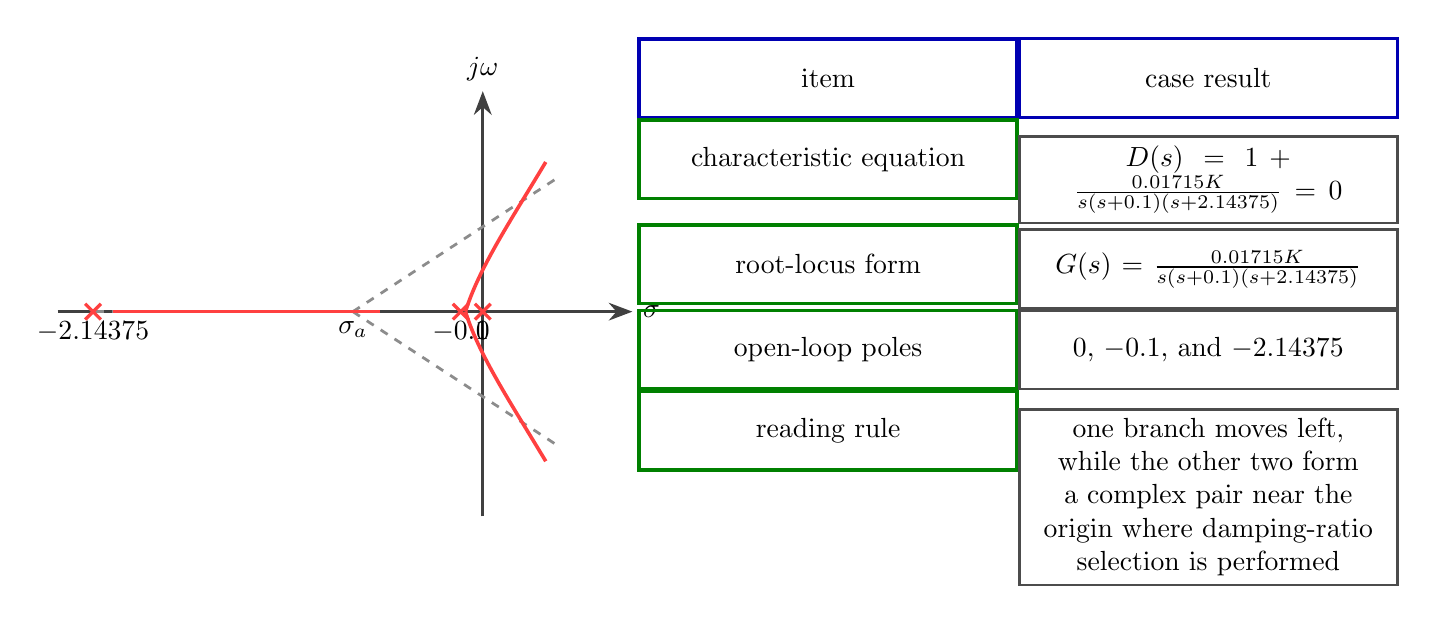
\begin{tikzpicture}
  \begin{scope}
    \draw[axis] (-5.4,0) -- (1.9,0) node[right] {$\sigma$};
    \draw[axis] (0,-2.6) -- (0,2.8) node[above] {$j\omega$};
    \draw[asym] (-1.65,0) -- (-5.0,0);
    \draw[asym] (-1.65,0) -- (0.95,1.7);
    \draw[asym] (-1.65,0) -- (0.95,-1.7);
    \draw[rl] (-4.7,0) -- (-1.3,0);
    \draw[rl] (-0.22,0) .. controls (-0.05,0.55) and (0.35,1.15) .. (0.8,1.9);
    \draw[rl] (-0.22,0) .. controls (-0.05,-0.55) and (0.35,-1.15) .. (0.8,-1.9);
    \foreach \x/\label in {0/{0},-0.28/{-0.1},-4.95/{-2.14375}} {
      \draw[pole] (\x-0.10,-0.10) -- (\x+0.10,0.10);
      \draw[pole] (\x-0.10,0.10) -- (\x+0.10,-0.10);
      \node[below] at (\x,0) {$\label$};
    }
    \node[below] at (-1.65,0) {$\sigma_a$};
  \end{scope}

  \begin{scope}[xshift=6.8cm]
    \matrix[matrix of nodes, nodes in empty cells, row sep=-\pgflinewidth, column sep=-\pgflinewidth] {
      \node[head] {item}; & \node[head] {case result}; \\
      \node[left] {characteristic equation}; & \node[cell] {$D(s)=1+\frac{0.01715K}{s(s+0.1)(s+2.14375)}=0$}; \\
      \node[left] {root-locus form}; & \node[cell] {$G(s)=\frac{0.01715K}{s(s+0.1)(s+2.14375)}$}; \\
      \node[left] {open-loop poles}; & \node[cell] {$0$, $-0.1$, and $-2.14375$}; \\
      \node[left] {reading rule}; & \node[cell] {one branch moves left, while the other two form a complex pair near the origin where damping-ratio selection is performed}; \\
    };
  \end{scope}
\end{tikzpicture}
\end{document}
